Tal y como se comentaba en la introducción, el código de partida del simulador contenía una única carpeta con el código principal muy extenso,  donde se encontraban los parámetros de la simulación,  la estructura  y los parámetros del estimador, los errores de la simulación... Dentro de esta, habia otra carpeta en la que se guardaba el propio programa de simulación, que se llamaba desde el programa principal. Es decir, el simulador inicial habia sido desarrollado con una filosofia de Sphagetti-coding. NO contaba con una estructura que facilitase ni la comprensión del propio código, ni mucho menos la implementación de posibles mejoras al mismo. De este modo, se decidió reestructurar el código en módulos siguiendo un paradigma de  programación imperativa para poder posterirmente proceder a implementar diferentes fumciones y modulos.


Actualmente, el código reestructurado cuenta con un código principal al que se accdede a través de uno más user-friendly (\textit{SimConfig.m}), y con varios módulos organizados en subcarpetas:
\begin{itemize}
    \item Estimation Module: en él se encuentran las funciones empleadas como estimador. Actualmente, el uníco estimador propuesto ha sido el UKF, pero de añadirse otros en un futuro se ubicarían aqui.
    \item Physics Module: contiene las funciones que representarán matemáticamente la fisica del problema que se pretende simular: la propagación de la órbita, las efemérides del sol\dots
    \item Simulation Module: en el se encuentra el código que corre la simulación como tal (\textit{Data\_Simulation.m}), así como el que genera el tipo de satélite deseado (\textit{Satellite.m}).
    \item Photometry module: incorpora las funciones que se desarrollan en la \autoref{s: fotometria}
    \item Utilities module: contiene varias funciones básicas necesarias para el correcto desarrollo del programa, funciones de cambio de ejes, pasar de cuaterniones a matrices de rotación\dots
\end{itemize}


\section{Funcionamiento del programa}

Como se venía comentando, el programa cuenta con 2 partes principales: el simulador y el estimador. Estos dos módulos se ejecutan consecutivamente al ser llamados desde el programa principal, donde se introducen los parámetros principales de la simulación, establecidos en el \textit{Sim\_config.m}. Estos incluyen el tamaño, actitud y posición inicial de la debris objetivo, el número de observadores y la altitud de los mismos y parámetros de la simulación como son la duración o la fecha de inicio de la misma, como se puede ver en el siguiente fragmento de código 

\begin{lstlisting}[language=Python, caption= Parámetros introducidos al programa principalen el \textit{Sim\_config.m}.]
    % Global Constants
    mu=3.986044418e14;
    Rt = 6878000;
    
    % Debris Parameters
    sim_params.sat_size = 2;   
    sim_params.sub_cat = 3;    
    sim_params.deploy_panels = 0;   
    sim_params.rt_init = [500, 0, 0]*1000 + Rt;
    sim_params.qt = [-0.401437297624753;-0.578215887659600;0.239454457519217;0.668712229668289];
    
    % Observers Parameters
    sim_params.n_observers = 5;  %
    sim_params.d_1stObs_target = 200000;
    sim_params.ro_init = [750, 0, 0] * 1000 + Rt;
    
    % Simulation Parameters
    sim_params.total_sim_time = 2*pi*sqrt(sim_params.ro_init(1)^3/mu);   
    sim_params.Year = 2023;
    sim_params.Month = 2;
    sim_params.Day = 25;
    sim_params.Hour = 15;
    sim_params.Min = 0;
    sim_params.Sec = 17;
\end{lstlisting}



\subsection{Desarrollo de la simulación}
Cuando el \textit{Main\_program.m} llama al simulador, se cargan en el mismo los parámetros establecidos anteriormente (amen de los pasos de tiempo que definen la simulación). A continuación, partiendo de la posición del target y de los datos del observador se utilizan dos funciones para situar los observadores en unas posiciones orbitales que permitan ver el target. 

A priori se decidió colocar todos los observadores en una misma órbita coplanaria a la del target como se puede observar en \autoref{fig: orbitas-coplanarias}, siguiendo la estructura de constelación expuesta en \cite{constellations}. Esto se consiguió desarrollando dos funciones de posicionamiento, una primera (\textit{generate\_position\_1st\_obs.m}), que crea el primer observador en la órbita especificada desde el fichero de configuración, ubicándolo a una distancia angular $\alpha$ del target, con el fin de asegurar la observación. 
\begin{figure}[H]
    \centering
    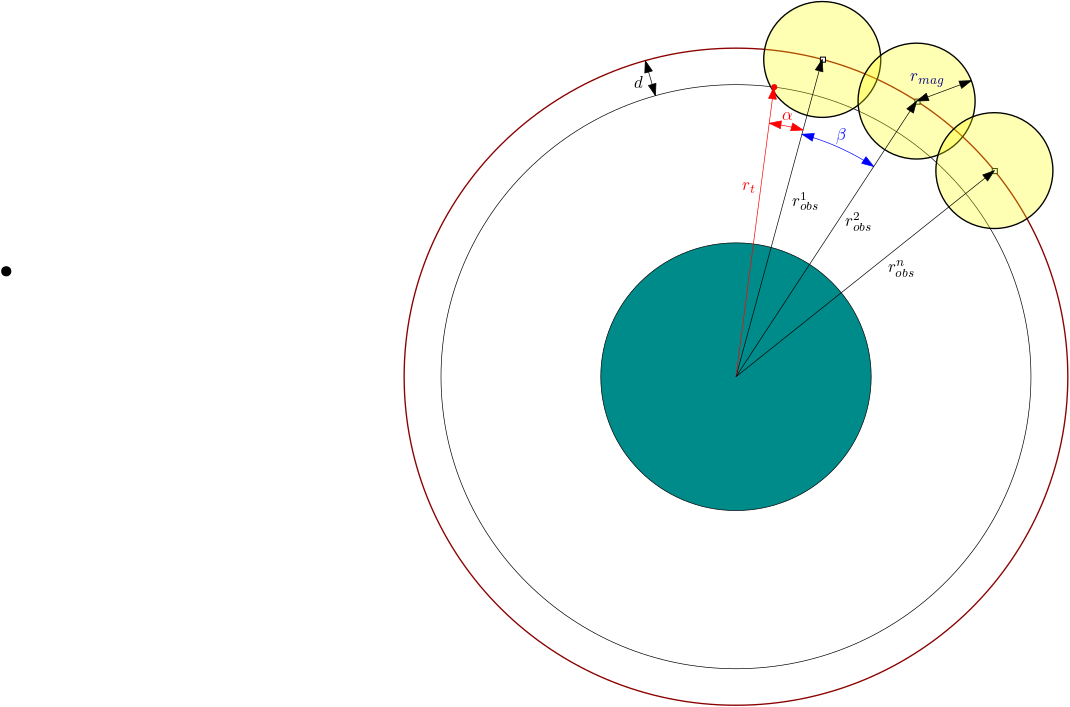
\includegraphics[width=0.6\columnwidth]{Figures/orbitas.png}
    \caption{Observers and target orbits configuration}
    \label{fig: orbitas-coplanarias}
\end{figure}
De manera análoga, se creó otra función (\textit{generate\_position\_N\_obs.m}) con el fin de colocar, en esta misma órbita al resto de observadores, dejando una distancia angular $\beta$ entre ellos. Nótese que ambas distancias quedarán subrrogadas al alcance de observación del sensor, definido en la simulación como el radio de la esfera de visibilidad.


Partiendo de la posición inicial de los observadores y el target, se propagan cada una de sus órbitas siguiendo la ecuación de las órbitas keplerianas mediante un esquema numérico Runge-Kutta 4:
\begin{aligned}
    &X_{n+1} =X_n+\frac {\Delta t}{6}\left(k_1+2k_2+2k_3+k_4\right),  \\
    &t_{n+1} =t_n+\Delta t , \quad, with n=0, 1, 2, 3...,
\end{aligned}
where $X$ represents the state vector, $t$ denotes time, and $k_1, k_2, k_3,$ and $k_4$ are intermediary values calculated as per the Runge-Kutta method,
\begin{aligned}
    &k_{1} =f(t_{n},X_{n}),  \\
    &k_{2} =f\biggl(t_{n}+\frac{\Delta t}{2},X_{n}+\Delta t\frac{k_{1}}{2}\biggr),  \\
    &k_{3} =f\biggl(t_{n}+\frac{\Delta t}{2},X_{n}+\Delta t\frac{k_{2}}{2}\biggr),  \\
    &k _4=f(t_{n}+\Delta t,y_{n}+\Delta tk_{3}). 
    \end{aligned}
Una vez propagadas las órbitas, se les añade un error acotado de posicionamiento, actitud y direccionalidad tanto al observador como al target, con el fin de simular la desviación que pueda haber en la medida real. Estos datos, así como los mismos sin el error se guardan como output del simulador, puesto que servirán a continuación como input del estimador.


Como se comentaba en la introducción, uno de los resultados clave de los los SSA system es la estimación del tamaño y la posición (ya sea mediante parámetros keplerianos, coordenadas cartesianas u otros) del RSO, ya que conociendo estos parámetros se puede predecir  con cierto nivel de precision la posición que tendrá el RSO en el futuro. Para ello se ha utilizado una versión reducida del algoritmo expuesto en \cite{linares}, en el que se estiman las variables presentes en el ector de estado $X$. 
Por el momento, por algunos de los motivos expuestos en \cite{UKFvsEKF}, se ha decidido usar el UKF, cuya formulación se va a describir a grandes rasgos a continuación. No obstante, como se ha comentado ya, gracias a la nueva estructura modular que ha adquirido el código, cambiar el estimador sería tan facil como incluir una función de estimación diferente en la carpeta.

\paragraph{Formulación del UKF}
Se considera el siguiente sistema no-lineal:
\begin{equation}\begin{aligned}\boldsymbol{x}_{k+1}&=f(\boldsymbol{x}_k,\boldsymbol{v}_k)\\\boldsymbol{y}_{k+1}&=h(\boldsymbol{x}_{k+1},u_k)\end{aligned}\end{equation}
 
donde $f(\boldsymbol{x})$ es la función que modeliza la evolución de las variables de estado (en el caso que nos atañe sería la \autoref{eq:state}),  $\boldsymbol{y}$ la s mediciones del sistema, $h$ la función de medida, $v, u$ lso errores de proceso y de medición respectivamente y $k$ un instante de tiempo arbitrario.

Asumiendo que la matriz de covarianza de las variables de estado ($\boldsymbol{P}_k$) es conocida (o estimada con cierto nivel de precisión) en ese instante, los sigma-points se  pueden calcular según,

\begin{equation}\begin{aligned}
    &\chi_{k}^{0} =x_{k}  \\
    &\chi_{k}^{i} =\boldsymbol{x}_k+\left(\sqrt{(n+\lambda)\mathbf{P}_k}\right)_i\quad i=1...n  \\
    &\chi_{k}^{i} =x_{k}+\left(\sqrt{(n+\lambda)\mathbf{P}_{k}}\right)_{i-n}\quad i=n+1\ldots2n, 
\end{aligned}\end{equation}
donde $\chi$ son los sigma-points, $n$ la dimensión del vector de estado y $\lambda$ un parámetro de escala que se calcula según,
\begin{equation}
\lambda = \alpha^2(n+\kappa)-n,
\end{equation}
donde $\alpha$ y $\kappa$ son a su vez parámetros que se deben ajustar de acuerdo a las necesidades del filtro. A continuación, se calculan los pesos asociados a los puntos sigma $W$:
\begin{equation}\begin{aligned}W^{0,m}&=\frac\lambda{\lambda+n}\\W^{0,c}&=\frac\lambda{\lambda+n}+1-\alpha^2+\beta\\W^{i,m}&=W^{i,c}=\frac\lambda{2(\lambda+n)}\quad i=1...2n\end{aligned},\end{equation}
donde $\beta$ es otro parámetro del estimador. 

Para usar el filtro de la manera más general posible, es conveniente que las medidas que tenga sean independientes de los sensores que las toman, ya que de lo contrario habria que modelizar el error introducido por cada uno de los equipos. Es por esto que se decide preproesar las medidas obtenidas realmente (en este caso las de la simulación), para pasar de los píxeles de luz quecaptarían los sensores a una medida más con más relevancia para el problema y que evita la introducción de ruido de los diversos equipos. Estas medidas son el vector unitario que apunta al RSO $\hat{\rho}$  y la magnitud aparente $m$.